\title{Study Guide for Midterm 1}
\author{Dr. Jordan Hanson - Whittier College Dept. of Physics and Astronomy}
\date{\today}
\documentclass[10pt]{article}
\usepackage[a4paper, total={18cm, 27cm}]{geometry}
\usepackage{outlines}
\usepackage{graphicx}
\begin{document}
\maketitle

\textbf{Instructions:} Work each problem \textit{before} checking your answer with the key (to follow on Moodle). \\ \vspace{0.25cm}

\section{Memory Bank}

\begin{enumerate}
\item Coulomb Force: $\vec{F} = k \frac{q_1 q_2}{r^2}\hat{r}$
\item $k = 9 \times 10^{9}$ N C$^{-2}$ m$^{2}$
\item $q_e = 1.6 \times 10^{-19}$ C
\item Mass of a proton: $1.67 \times 10^{-27}$ kg
\item Atomic mass: the number of grams per mole of a substance
\item Avogadro's number: $6.03 \times 10^{23}$ molecules or atoms
\item Electric field and charge: $\vec{F} = q \vec{E}$
\item Field of two oppositely charged infinite planes, with charge density $\sigma$: $\vec{E}(z) = \frac{\sigma}{\epsilon_0}\hat{z}$
\item $\epsilon_0 \approx 8.85 \times 10^{-12}$ F/m
\item Potential energy and voltage: $U = q\Delta V$
\item 1 eV: an electron-Volt is the amount of energy one electron gains through 1 V.
\item Voltage of a point charge: $V(r) = k\frac{q}{r}$
\item Voltage and E-field: $\vec{E} = -\frac{\Delta V}{\Delta x}$
\item Voltage between two oppositely charged infinite planes: $V(x) = -E x + V_0$
\item Capacitance: $Q = CV$
\item Parallel plate capacitor: $C = \frac{\epsilon_0 A}{d}$
\item Adding two capacitors in \textit{series}: $C_{tot}^{-1} = C_1^{-1} + C_2^{-2}$
\item Adding two capacitors in \textit{parallel}: $C_{tot} = C_1 + C_2$
\end{enumerate}

\section{Electric Charge and Electric Fields}

\begin{enumerate}
\item (a) A certain lightning bolt moves 40.0 C of charge.  To how many electrons does this correspond? (b) Suppose a speck of dust in an oil drop experiment\footnote{A great paper topic, by the way: the Millikan oil drop experiment.} has  $10^{12}$  protons in it and has a net charge of -5.00 nC (a very large charge for a small speck). How many electrons does it have?\\ \vspace{1cm}
\item (a) Two charges exert $F_{\rm C} = 5.00$ N of force on each other. What will $F_{\rm C}$ be if the distance between them triples? (b) If one charge is $1 nC$, and the other is $2 nC$, what is the distance between them if $F_{\rm C} = 5.00$ N? \\ \vspace{1cm}
\item 
\begin{figure}
\centering
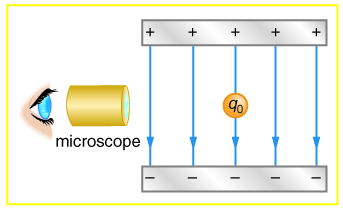
\includegraphics[width=0.5\textwidth]{mill.jpeg}
\caption{\label{fig:mill} The classic Millikan oil drop experiment was a measurement of the charge of an electron.}
\end{figure}
The classic Millikan oil drop experiment was the first to obtain an accurate measurement of the charge on an electron. In it, oil drops were suspended against the gravitational force by a vertical electric field. (See Fig. \ref{fig:mill}.) Given the oil drop to be $1.0 \mu$m in radius and have a density of 920 kg/m$^3$: (a) Find the weight of the drop. (b) If the drop has a single excess electron, find the electric field strength needed to balance its weight. \\ \vspace{1.75cm}
\item Suppose two positive, identical charges are located a distance $d$ apart. (a) Sketch the electric field below.  (b) Sketch the electric field if instead one of the charges is negative. \\ \vspace{1.5cm}
\end{enumerate}

\section{Potential Energy and Voltage}

\begin{enumerate}
\item What is the electric field across an 10.00 nm thick membrane if (a) the voltage across it is 50 mV? You may assume a uniform electric field. (b) Suppose this cell membrane is part of a nerve cell.  How much energy would an electron gain if dropped through the 50 mV voltage and accelerated across the cell freely?  Express your anser in electron-Volts (eV). \\ \vspace{1.25cm}
\end{enumerate}

\section{Capacitors}

\begin{enumerate}
\item ff
\end{enumerate}

\end{document}